\documentclass[tikz, border=10pt]{standalone}

\usepackage{tikz}
\usepackage{pgfplots}
\pgfplotsset{width=10cm, compat=1.9}

\begin{document}
    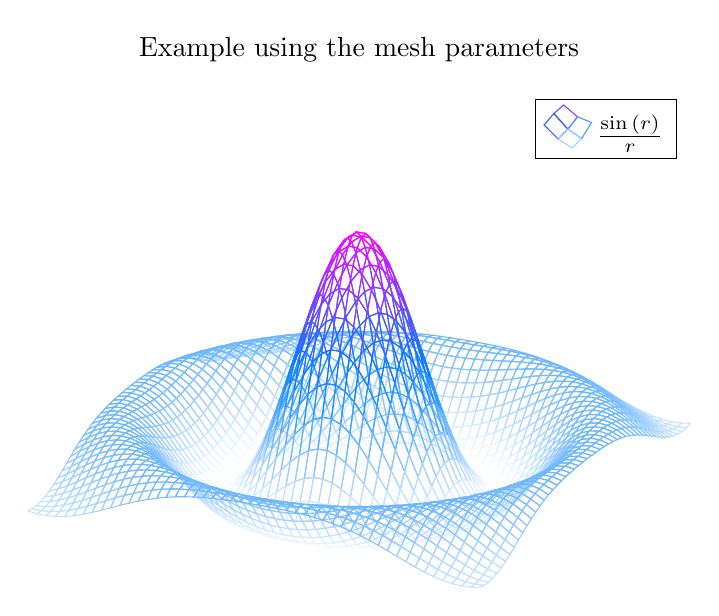
\begin{tikzpicture}
        \begin{axis}[
            title={Example using the mesh parameters},
            hide axis,
            colormap/cool
        ]
            \addplot3[mesh, domain=-8:8, samples=50]{sin(deg(sqrt(x^2 + y^2)))/sqrt(x^2 + y^2)};
            \addlegendentry{$\frac{\sin{(r)}}{r}$}
        \end{axis}
    \end{tikzpicture}
\end{document}